\documentclass[10pt,a4paper]{article}
\usepackage[margin=2cm]{geometry}\usepackage{graphicx,booktabs,hyperref,float}
\title{Memory Pressure in Virtualized Ubuntu and Adaptive Page Replacement under Workload Shift}
\author{Ripti \\ Dept. of CSE, MIST \\ CSE-307 Operating Systems}
\date{}
\begin{document}\maketitle
\begin{abstract}
(3--4 sentences: what you ran, main finding on RAM vs runtime/swap, main finding on which policy degraded most.)
\end{abstract}
\section{Introduction}
Virtual machines expose vRAM/vCPU abstractions mapped onto finite host resources \cite{popek,waldspurger,hasan}. When the working set exceeds vRAM, the guest OS pages to swap \cite{silberschatz,tanenbaum}. Part A measures this on VMware; Part B studies replacement policies FIFO, LRU and Belady's optimal \cite{belady} plus a learned policy under a workload shift.
\section{Experimental Setup}
\textbf{Part A.} Host: (CPU, RAM, VMware version). Guest: Ubuntu (version). Workload: 4 processes, 1536\,MB total working set, sequential then 400k random page touches per process (\texttt{workload.py}), identical in all runs. Configurations: RAM $\in\{1,2,4\}$\,GB $\times$ vCPU $\in\{1,2,4\}$, 5 repetitions each; caches and swap cleared before each run. Metrics: wall time, major/minor faults, swap-out pages (\texttt{/proc/vmstat}), CPU\%.\\
\textbf{Part B.} 200 pages, 16 frames, 20{,}000 references; first half looping over 24 hot pages, second half random with bursts. Learned policy: logistic regression \cite{sklearn} on age, log-age, access count, recent frequency, predicting ``page not reused soon''; the page with highest score is evicted. \emph{Static} model trained on pre-shift data only; \emph{adaptive} model retrained every 500 references. 10 random seeds.
\section{Results}
\begin{figure}[H]\centering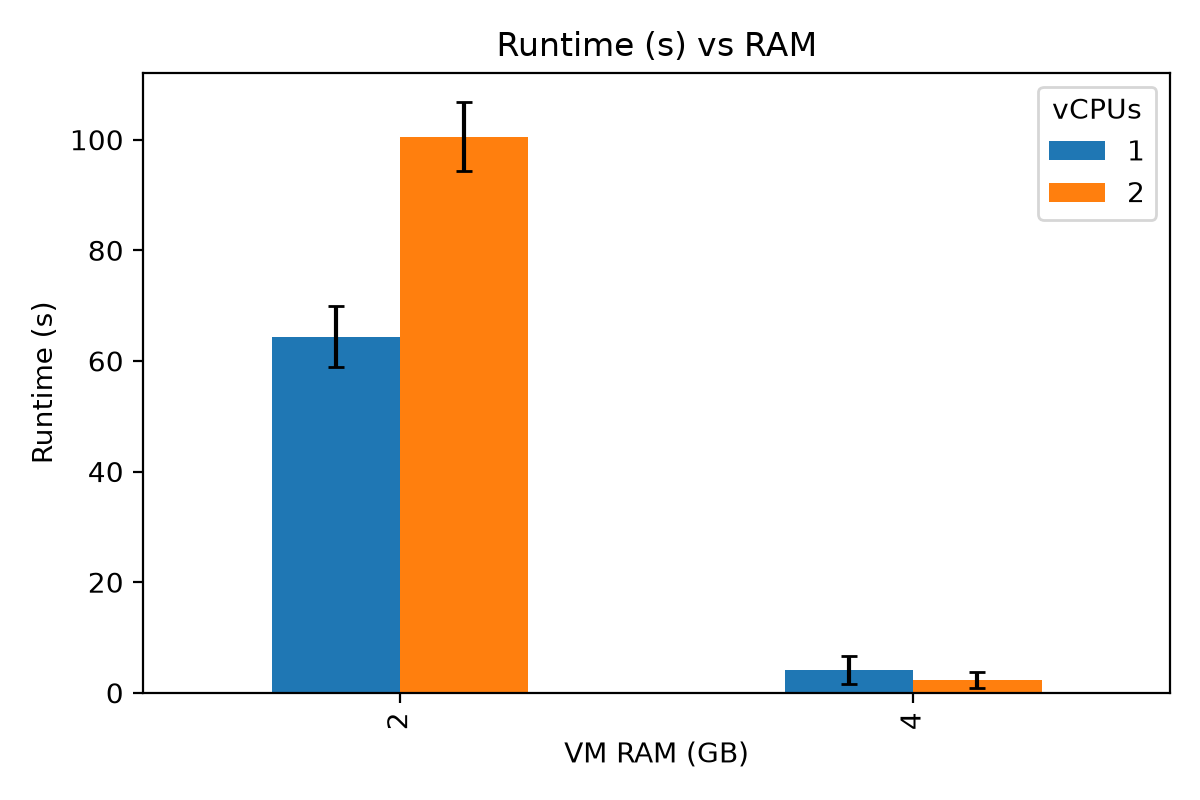
\includegraphics[width=.48\linewidth]{../results/vm_runtime.png}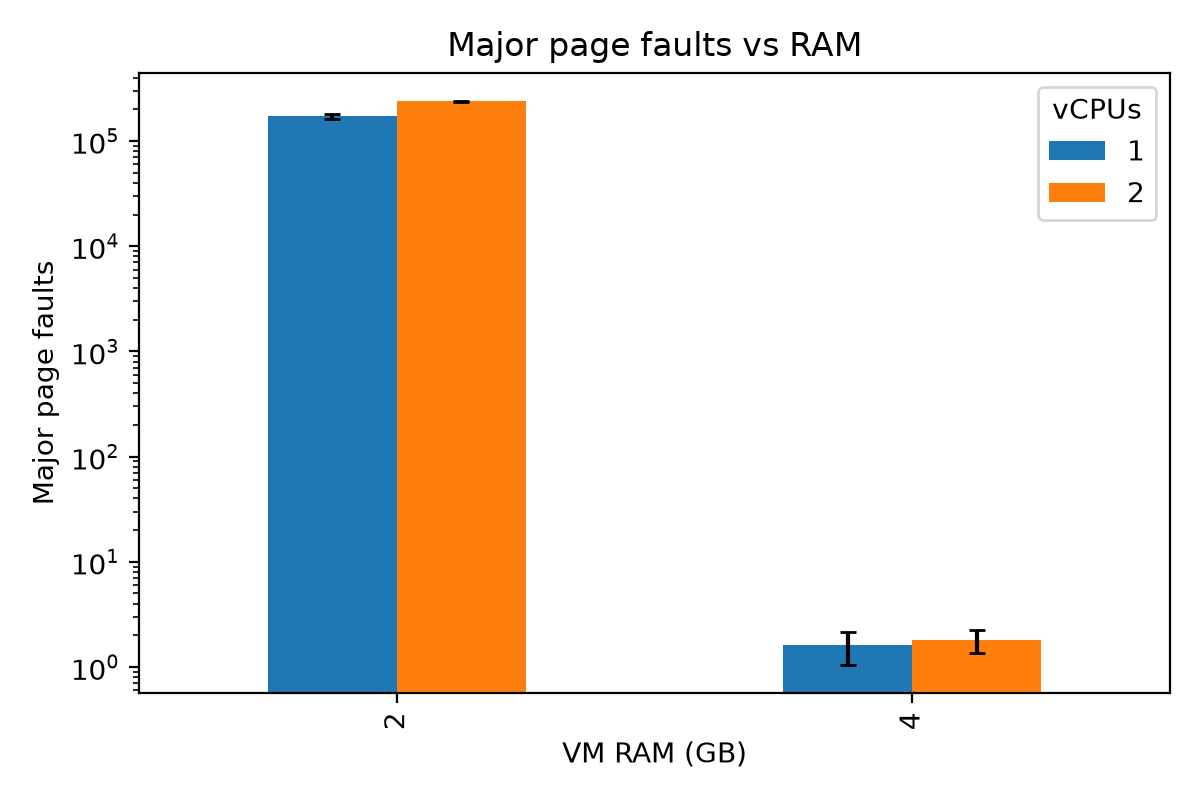
\includegraphics[width=.48\linewidth]{../results/vm_majflt.png}\caption{Runtime and major faults vs VM RAM.}\end{figure}
(Insert table from vm\_summary.csv; 2--3 sentences.)
\begin{figure}[H]\centering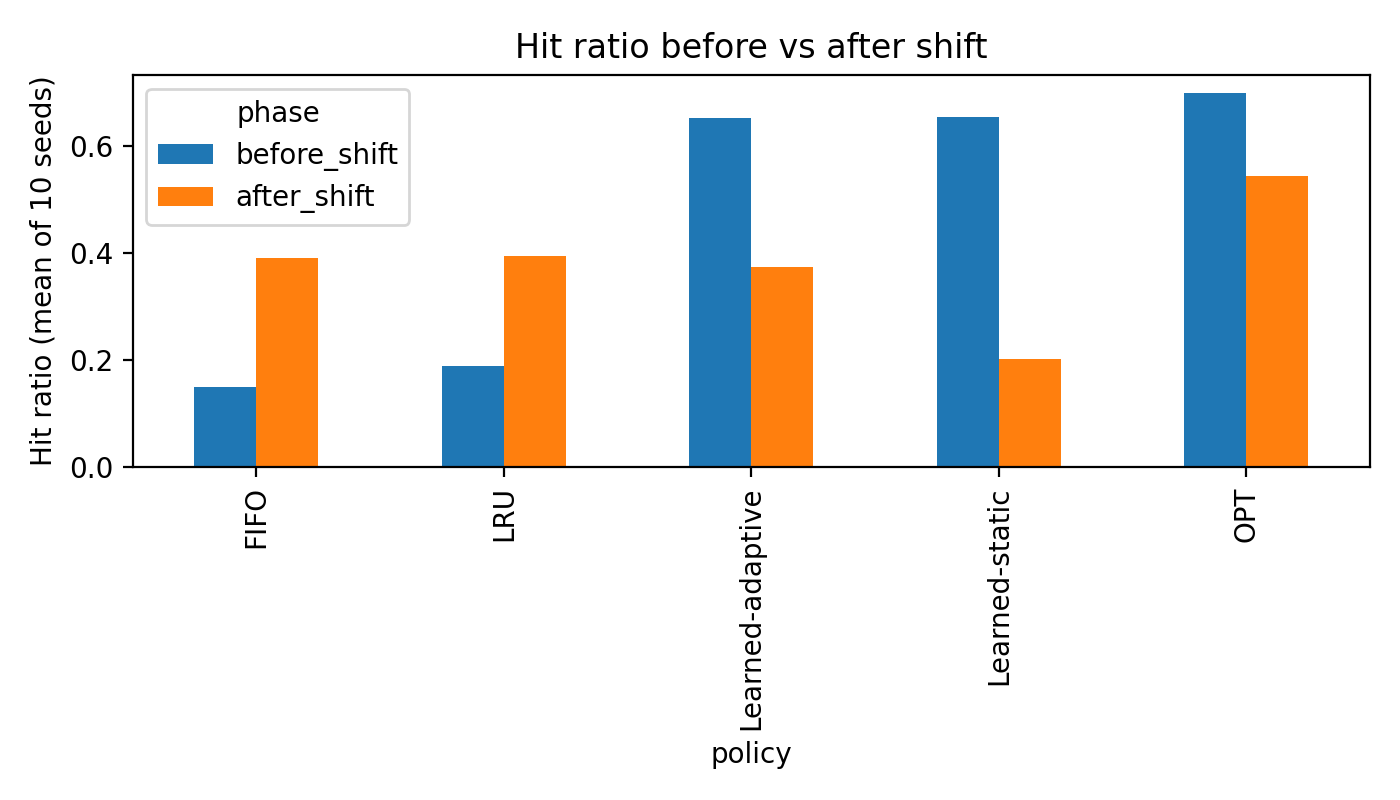
\includegraphics[width=.48\linewidth]{../results/page_hit_ratio.png}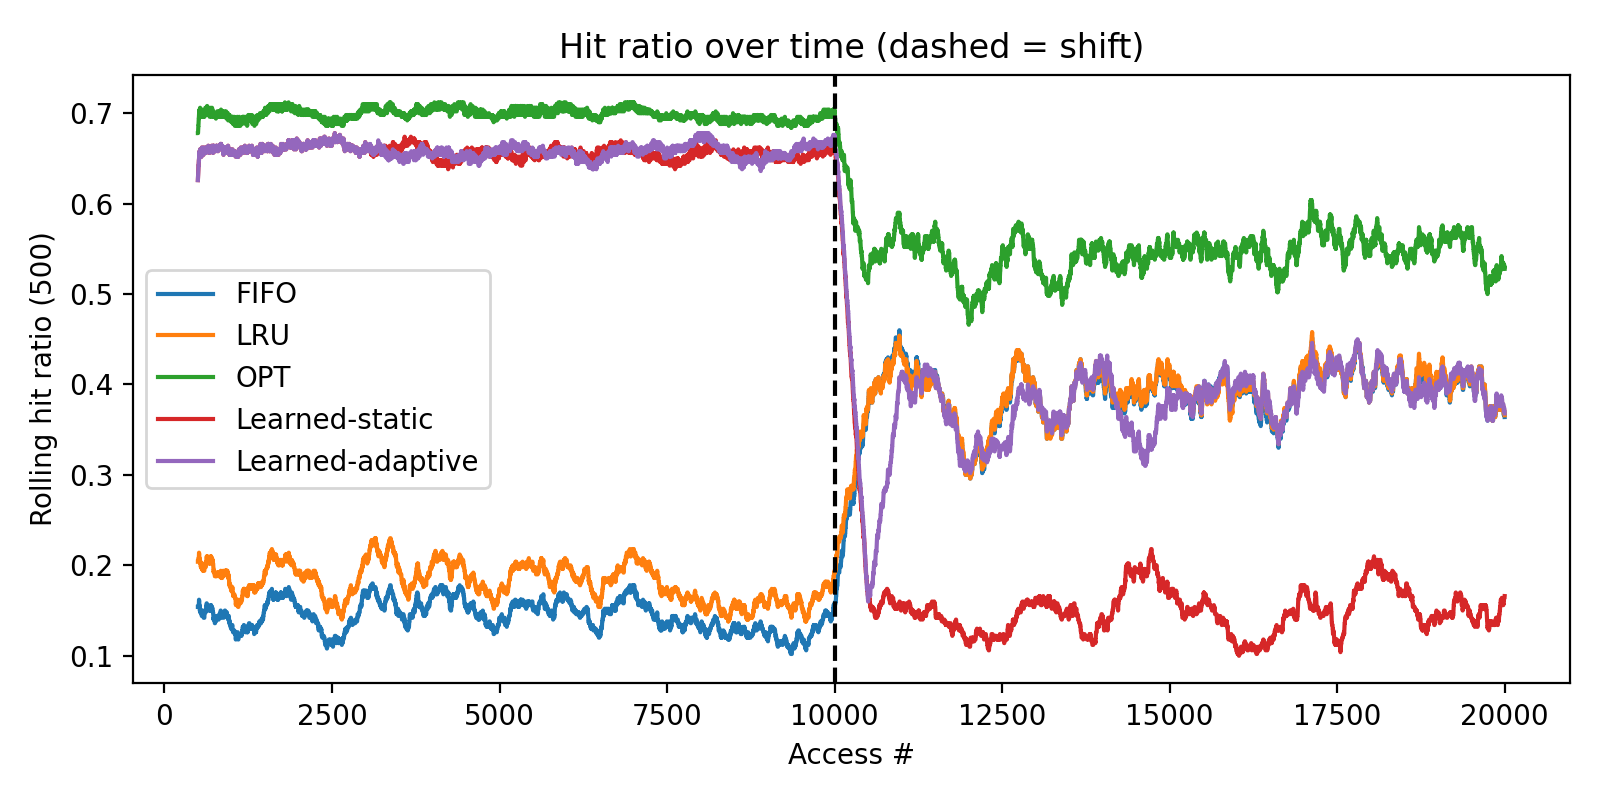
\includegraphics[width=.48\linewidth]{../results/page_rolling.png}\caption{Hit ratio before/after shift; rolling hit ratio.}\end{figure}
(Insert page\_degradation.csv as table.)
\section{Analysis}
\textbf{Virtualization link:} vRAM below working set $\Rightarrow$ swapping, thrashing; vCPU count vs host cores; overcommitment and ballooning \cite{waldspurger}. \textbf{Page replacement:} LRU/FIFO collapse on a loop larger than the frame count (24 pages $>$ 16 frames); the static learned model wins pre-shift but degrades most after the shift because its training distribution changed; retraining recovers part of the loss; OPT is the upper bound.
\section{Limitations and Conclusion}
(Synthetic trace, small VM count, no real page-fault trace, nested virtualization noise.)
\bibliographystyle{plain}\bibliography{refs}
\end{document}
